\chapter{Analysis of the Outer Detector} \label{chap:analysis_of_the_od}

\par
In this chapter, the calibration of the OD, once it was constructed is described, which sets the foundations for assessing if the requirements set out in \autoref{tab:veto_requirements} are achieved.
These requirements are: that the neutron veto efficiency is at least 95\%, and that no more than 5\% of the WIMP search time is vetoed.
\par
For ascertaining an appropriate veto window, a study on the OD backgrounds is performed. 
This is followed by the results from a neutron calibration.
Together these provide the assessment of the performance.
\par
Finally a particle discrimination method is suggested, which in future may allow for the OD to be used as a more intelligent veto.


%\section{OD Energy Scale} \label{sec:od_energy_scale}
\par
After construction and the filling of the OD, the SPE for each PMT was checked using the OD optical calibration system (OCS) described in \cite{lz_ocs_system_ref}.
A detailed description of the PMT monitoring during the commissioning and SR1 can be found in the works of E. Fraser \cite{ewanfraser_thesis_ref}. 
\par
During this period, an energy calibration of the OD was performed.
Again, details of the methodology are described in \cite{ewanfraser_thesis_ref} but summarised below.
As mentioned in Sec. \ref{sec:lz_detector_chapter}, a variety of calibration sources were available with output a range of particles at different energies.
$\gamma$ sources were lowered into the CSD's to the 700mm level (see Fig. \ref{fig:CSD1_Geometry}) and the number of photo electrons measured.
The empirical formula for the non-linear energy response of the scintillator from DayaBay \cite{dayabay_antineutrino_oscillation_ref, ls_nonlinear_energy_response_ref}, shown in Eq. \ref{eq:ls_light_response}, was used to fit to these points.
\begin{equation}
    \frac{E_{vis}}{E_{true}} = \frac{p_0  + p_3 \times E_true}{1 + p_1 \times e^{p_2 \times E_{true}}}
    \label{eq:ls_light_response}
\end{equation}
The fit and the translation from photons detected to energy are shown in Fig. \ref{fig:od_energy_scale}.

\begin{figure}[]
    \centering
   \begin{tikzpicture}
    \begin{groupplot}[%view={0}{90},
    group style = {group size = 1 by 2,vertical sep=0.5cm},
                   width=0.98\textwidth]
    \nextgroupplot[
            ylabel=LS energy response ($\frac{E_{vis}}{E_{true}}$),
            %xlabel=,
            xticklabels={,,}
            height=10cm, width=\textwidth,
            xmin=0, xmax=10,
            grid=major,
            ]
            %\addplot[black, smooth, domain=0:10] 
                    %{(0.00535 + 0.0286*x) / (1-0.9918*exp(-0.03018*x))};
                    %{((0.001894 + 0.03614*x) / (1-1*exp(-0.001453*x)))};
            \addplot[black, smooth]
                table[x=Energy,y=Value]
                {Data/OD_Energy_Scale/emperical_fit.dat};
                    
            \addplot[only marks,
                 error bars/.cd,
                 y dir=both, y explicit, error bar style={color=black}] table[x=Energy,y=light_response, y error=light_response_Error] {Data/OD_Energy_Scale/phd_energy.dat};

    \nextgroupplot[
            ylabel=N. photons detected,
            xlabel=Energy (MeV),
            height=6cm, width=\textwidth,
            xmin=0, xmax=10,
            ymin=0, 
            grid=major,
            ]
            \addplot[only marks,
                 error bars/.cd,
                 y dir=both, y explicit, error bar style={color=black}] table[x=Energy,y=pulseArea, y error=pulseArea_Error] {Data/OD_Energy_Scale/phd_energy.dat};
            \addplot[black, smooth, domain=0:10] 
                    {-33.98 + 0.2425*x*1000};
            
  \end{groupplot}
    \end{tikzpicture}
    \caption{OD Energy Scale and the relation between observed number of photons and the energy deposited. Analysis by E. Fraser \cite{ewanfraser_thesis_ref}.}
    \label{fig:od_energy_scale}
\end{figure}

%    \nextgroupplot[
%            ylabel=N. photons detected,
%            xlabel=Energy (MeV),
%            height=6cm, width=\textwidth,
%            xmin=0, xmax=10,
%            ymin=0, 
%            grid=major,
%            ]
%            \addplot[black]
%                    table [x=Energy,y=Value]
%                    {Data/OD_Energy_Scale/phd.dat};

\par
The fit 
Although this provides a good result for SR1, as the calibrations were only performed at a single position, the varying light collection efficiency around the OD was not taken into account (see Fig. \ref{fig:od_lce}).



%\section{Backgrounds}
\label{sec:od_analysis_backgrounds}
\par
Using the aforementioned energy scale, noise cut, and scaling factor, in this section the background rate in the OD is measured and attempts are made to understand what is seen.
\par
In \autoref{fig:od_random_trigger} a comparison between the observed events in the OD during the entirety of SR1 and those expected are shown from the Random Trigger.
The expected rates are those described in \autoref{sec:simulated_od_requirements} and were simulated using the ``full-propagation" chain with the result scaled by the factor determined in the previous section.
Both data and simulations were handled by the same analysis tools, with the noise cut applied to both.
Included as well in \autoref{fig:od_random_trigger} is the expected rate in the OD if the GdLS had not undergo an improve purification.
Neither case fits what is observed particularly well.
More worryingly there is a peak in the data at 100 phd which does is not in the expected rate.


\begin{figure}[]
    \centering
    \begin{tikzpicture}
    
    \begin{axis}[
        xlabel=Pulse Area,
        ylabel=Rate (Hz/5phe),
        width=15cm, height=10cm,
        xmin=0, xmax=1000,
        %ymax=1e-7, 
        ymode=log,
        legend pos=north east,
        grid=major]
            
        \addplot[only marks, mark size=0.5pt,
                 error bar legend,] 
            plot[error bars/.cd, x dir=both, x explicit]
            table[x=pulsearea,y=weight,x error=xerror, y error=yerror]
            {Data/OD_Backgrounds/background_constraints/od_data.dat};
        
        \addplot[red, const plot]
            table [x=pulsearea,y=weight]
            {Data/OD_Backgrounds/background_fit/starting_point/backgrounds_improved_purification.dat};
            
        \addplot[green, const plot]
            table [x=pulsearea,y=weight]
            {Data/OD_Backgrounds/background_fit/starting_point/backgrounds_original_purification.dat};
        
        \legend{Data, Original purification, Improved purification};
        \end{axis}
    \end{tikzpicture}
    \caption{OD pulse area spectrum from using the Random Trigger in the region. 
    Only the noise cut has been applied to the data.
    Overlaid are the expected rates from all backgrounds with the improved and original GdLS internal rates.}
    \label{fig:od_random_trigger}
\end{figure}

\par
In the remainder of this section, an attempt is made to understand what is observed and why it is different to what is expected.

\subsection{Rate Stability}

\par
To begin in the journey of understanding what is in the data, the first thing that was done was observe if the rate and distribution were stable over time.
Events from a month before the beginning of SR1 until the end were monitored every week using the Random Trigger.
The rate of events above the noise-cut, 100 keV and 200 keV were measured and are shown in \autoref{fig:OD_SR1_Rate}.
The noise-cut was applied as a base-cut, so the 100 keV is made up of the the noise-cut plus a phd cut, and similarly for 200 keV.
The three gaps in the data are when a calibrations were being performed.
This occurred three times in the region shown: just before SR1, 4 weeks into SR1, and straight after SR1.
\par
There are minor fluctuations in the noise-cut rate, but these are linked a xenon chiller and is consistent with a grounding failure, thus the behaviour is not mirrored in the 100 keV or 200 keV rates.
Importantly, over this period the OD rate remains stable, with no features in the observed distribution changing during that time.
Therefore what was shown in \autoref{fig:od_random_trigger} is the truly representative of the backgrounds in the OD.

\begin{figure}[!htbp]
    \centering
   \begin{tikzpicture}
        \begin{axis}[
        date coordinates in=x,
        %xtick=data,
        xticklabel style=
        {rotate=90,anchor=near xticklabel},
        xticklabel=\day.\month.\year,
        xlabel={Date},
        %ymin=247, ymax=250,
        y tick label style={/pgf/number format/1000 sep=},
        extra y tick style={grid=major, tick label style={xshift=-1cm}},
        ylabel={Rate (Hz)},
        date ZERO=2009-08-18,% <- improves precision!
        width=15cm,
        height=6cm,
        ]
        \addplot[smooth, error bar legend,
                 error bars/.cd,
                 y dir=both, y explicit, error bar style={color=orange}] table[x=date,y=noise, y error=noise_error] {Data/OD_Backgrounds/background_rates/random_trig_rates.txt};
                 
        \addplot[smooth, error bar legend,
                 error bars/.cd,
                 y dir=both, y explicit, error bar style={color=orange}] table[x=date,y=100kev, y error=200kev_error] {Data/OD_Backgrounds/background_rates/random_trig_rates.txt};
        
        \addplot[smooth, error bar legend,
                 error bars/.cd,
                 y dir=both, y explicit, error bar style={color=orange}] table[x=date,y=200kev, y error=200kev_error] {Data/OD_Backgrounds/background_rates/random_trig_rates.txt};
                 
        \end{axis}
    \end{tikzpicture}
    \caption{Rate in OD during and before SR1 data taking on a week-by-week basis using the Random Trigger.
    Week -1 corresponds to the month prior to SR1 when the OD PMT gains were higher.}
    \label{fig:OD_SR1_Rate_spare}
\end{figure}
%\par


\begin{figure}[!htbp]
    \centering
    \begin{tikzpicture}
        \begin{axis}[
            title=TODO: Replace with dates and errors,
            xlabel=Data taking week,
            ylabel=Rate (Hz),
            width=15cm,
            height=6cm,
            xmin=-2,
            xmax=14,
            legend style = {column sep = 10pt, legend columns = -1,}]
            \addplot[red, only marks]
                    table [x=Week,y=Rate]
                    {Data/OD_Backgrounds/background_rates/od_sr1_rate_noise.dat};
            \addlegendentry{Noise Cut};
            \addplot[blue, only marks]
                    table [x=Week,y=Rate]
                    {Data/OD_Backgrounds/background_rates/od_sr1_rate_100.dat};
            \addlegendentry{100keV};
            \addplot[green, only marks]
                    table [x=Week,y=Rate]
                    {Data/OD_Backgrounds/background_rates/od_sr1_rate_200.dat};
            \addlegendentry{200keV};
        \end{axis}
    \end{tikzpicture}
    \caption{Rate in OD during and before SR1 data taking on a week-by-week basis using the Random Trigger.
    Week -1 corresponds to the month prior to SR1 when the OD PMT gains were higher.}
    \label{fig:OD_SR1_Rate}
\end{figure}

\par
Viewing the rate in a slightly different way, the rate-per-phd for the SR1 period is shown in \autoref{fig:od_sr1_rate_vs_threshold}.
Overlaid is the expected rate of backgrounds from \autoref{tab:od_expected_rates} for 100 and 200 keV.
Interestingly the rate above 100 keV is in fairly good agreement with what was predicted in \autoref{sec:simulated_od_backgrounds}.
This is consistent with being able to set the veto energy threshold to 100 keV, assuming that achieves an appropriate veto efficiency.
However differences arise at the 200 keV level, where the expected is 62.7$\pm$5.3 Hz were as the observed is 42.5$\pm$2.1 Hz, a fairly significant difference.

\begin{figure}[]
    \centering
    \begin{tikzpicture}
        \begin{axis}[
            xlabel=OD Threshold (phd),
            ylabel=Rate (Hz),
            width=15cm, height=8cm,
            xmin=-1, xmax=55,
            ymin=0, ymax=350,
            legend pos=north east,
            grid=major]
             \addplot+[black, smooth, mark=none]
                    table [x=Threshold,y=Rate]
                    {Data/OD_Backgrounds/background_rates/od_sr1_rate_vs_threshold_smooth_line.dat};
            \addplot[black, only marks, 
                     error bar legend,
                     error bars/.cd,
                     x dir=both, x explicit, error bar style={color=black}]
                    table [x=Threshold,y=Rate, x error=XError]
                    {Data/OD_Backgrounds/background_rates/od_sr1_rate_vs_threshold_error_bars.dat};
             \addplot[dashed, mark=none, red] coordinates {(0,100) (60,100)};
             \addplot[dashed, mark=none, blue] coordinates {(17.6,0) (17.6,350)};
             \addplot[dashed, mark=none, green] coordinates {(37.5,0) (37.5,350)};
             
             \addplot[orange, only marks, 
                      error bar legend,
                      error bars/.cd,
                      y dir=both, y explicit, error bar style={color=orange}]
                      table [x=Threshold,y=Rate, y error=YError]
                      {Data/OD_Backgrounds/background_rates/od_sr1_rate_expected.dat};
             
             \legend{,SR1 Data,$<$100Hz Requirement,100 keV (17.6 phd),200 keV (37.5 phd),Expected}                
        \end{axis}
    \end{tikzpicture}
    \caption{Rate of OD backgrounds during SR1 using the Random Trigger. The noise cut has been applied. 100Hz Requirement is for a 500$\mu$s veto window as proposed in \cite{LZ_TechnicalDesignReview_ref}. Expected values are from \autoref{tab:od_expected_rates}}
    \label{fig:od_sr1_rate_vs_threshold}
\end{figure}

%%%%%%%%%%%%
\subsection{Position Reconstruction}
\par
Next we can look at the spacial distribution of events.
For any pulse it is possible to reconstruct the location of the interaction that caused the pulse by a weighted average such as:
\begin{equation}
    x = \frac{\sum{\text{Ch}_{\text{phd}} * \text{Ch}_\text{x}}}{\sum{\text{Ch}_\text{phd}}} 
\label{eq:OD_xy_position}
\end{equation}
where Ch$_{phd}$ is the phd of a PMT channel and Ch$_{x}$ is the position of the PMT.
Due to scheduling constraints associated with SR1, there was an insufficient variety of calibration sources were used at varying \{$x,y,z$\} positions in order to adequately determine the resolution of this approach, but it is something a future calibration campaign may be able to tackle. 
Additionally, this approach does not take into account the OCV in the centre of the detector, so reconstructed pulses will have an incorrect position, but the correct shape.
The OCV can be taken into account by converting coordinate system, but has explicitly not been done here due to the lack of knowledge in the actual resolution of this approach.
Regardless however, this approach does provide an insight in a way not thought possible based upon optical simulations.

\par
This approach was performed on slices in phd-space, the result of which can be seen in \autoref{fig:od_backgrounds_position_reconstruction}.
The first region focuses on the peak at 100 phd ($\backsim$ 0.5 MeV).
The second region focuses on the area above 2 MeV, where cavern-$\gamma$s should dominate.

\begin{figure}[!htbp]%
\centering
\begin{tikzpicture}
\centering
  \begin{groupplot}[%view={0}{90},
    group style = {group size = 2 by 3,vertical sep=3cm,
                   horizontal sep=1.5cm},
                   height=6cm, width=0.5\textwidth]
    \nextgroupplot[
            ylabel=Rate (Hz),
            xlabel=Pulse Area (phd),
            width=0.95\textwidth,
            height=6cm,
            %xshift=0.5\textwidth,
            xmin=0, xmax=800,
            ymin=1e-4, ymax=1e3,
            ymode=log,
            ]
            \addplot[only marks, mark size=1.0pt] 
            plot[error bars/.cd, x dir=both, x explicit]
            table[x=pulsearea,y=weight,x error=xerror, y error=yerror]
            {Data/OD_Backgrounds/background_constraints/od_data.dat};
            
            \addplot[dashed, mark=none, name path=A,blue] coordinates {(75,0.00001) (75,10000)};
            \addplot[dashed, mark=none, name path=B,blue] coordinates {(125,0.00001) (125,10000)};
            \addplot[dashed, mark=none, name path=C,green] coordinates {(500,0.00001) (500,10000)};
            \addplot[dashed, mark=none, name path=D,green] coordinates {(1000,0.00001) (1000,10000)};

            \addplot[blue!50] fill between[of=A and B];
            \addplot[green!50] fill between[of=C and D];
            
    \nextgroupplot[group/empty plot]

    \nextgroupplot[colorbar, 
    colorbar style={title=Rate (Hz),ymode=log,},
    width=0.4\textwidth, view={0}{90},
    xshift=-0.3\textwidth,
    ylabel=Z (cm),
	xlabel=R (cm),
	y label style={at={(axis description cs:-0.13,0.5)},anchor=near ticklabel},]
    \addplot3[
		surf,
		shader=flat corner,
		mesh/cols=50,
		mesh/ordering=rowwise,
		point meta = {z>1 ? nan : z}
		] file {Data/playground/alpha_peak_r_z.csv};
	\node [rotate=90] at (axis cs:0,1050) {Region 1};
	\nextgroupplot[colorbar, 
	colorbar style={title=Rate (Hz),ymode=log,},
	width=0.4\textwidth, view={0}{90},
    xshift=-0.5\textwidth, %yshift=1.5cm,
    ylabel=Y (cm),
	xlabel=X (cm),
	y label style={at={(axis description cs:-0.13,0.5)},anchor=near ticklabel},]
    \addplot3[
		surf,
		shader=flat corner,
		mesh/cols=54,
		mesh/ordering=rowwise,
		point meta = {z>1 ? nan : z}
		] file {Data/playground/alpha_peak_x_y.csv};

    \nextgroupplot[colorbar, 
    colorbar style={title=Rate (Hz),ymode=log,},
    width=0.4\textwidth, view={0}{90},
    ylabel=Z (cm),
	xlabel=R (cm),
	y label style={at={(axis description cs:-0.13,0.5)},anchor=near ticklabel},]
    \addplot3[
		surf,
		shader=flat corner,
		mesh/cols=50,
		mesh/ordering=rowwise,
		point meta = {z>1 ? nan : z}
		] file {Data/playground/rg_th232_r_z.csv};
		
	\nextgroupplot[colorbar, 
	colorbar style={title=Rate (Hz),ymode=log,},
	width=0.4\textwidth, view={0}{90},
	ylabel=Y (cm),
	xlabel=X (cm),
    y label style={at={(axis description cs:-0.13,0.5)},anchor=near ticklabel},]
    \addplot3[
		surf,
		shader=flat corner,
		mesh/cols=54,
		mesh/ordering=rowwise,
		point meta = {z>1 ? nan : z}
		] file {Data/playground/rg_th232_x_y.csv};
   
  \end{groupplot}
  
  \node at ($(group c1r2) + (-1.0cm, 3.5cm)$) {\textbf{Region 1 (blue)}};
  \node at ($(group c1r3) + (-1.0cm, 3.5cm)$) {\textbf{Region 2 (green)}};
  
\end{tikzpicture}
\caption{Position Reconstruction of pulses from various regions in pulse area space defined in the top plot. 
         Each pulse has had the noise cut applied and the position reconstructed using \autoref{eq:OD_xy_position}.}
\label{fig:od_backgrounds_position_reconstruction}
\end{figure}

\par
There are two useful observations in both regions.
Firstly, in $r-z$ there is a clear bias to events at the bottom of the detector.
This is consistent with cavern-$\gamma$s distribution shown in \autoref{fig:cavern_gamma_position_distribution}.
This indication that the cavern-$\gamma$s is the most significant contributor, again in agreement in the prediction (\autoref{tab:od_expected_rates}).
Secondly, in $x-y$ there is an elevated rate of events in \{$+x,+y$\}.
This can be understood easiest by labelling the SATs with letters A-D starting from \{$+x,+y$\} and going around clockwise.
Using this labelling, over the period of SR1, SAT A has a rate in excess of 8\% higher than any of the other tanks, with SAT B seeing the next highest rate (3\% higher than the mean).
Both SATs C and D saw an equivalent rate.
In \autoref{fig:OD_conduit_geometry}, the SAT placement are shown along with the conduits.
SAT A and SAT B are the only tanks which are obstructed by a single conduit, additionally both tanks cover an entire BAT and TAT.
The CSD-ports and the OCV legs block the other SATs from the TATs and BATs.
This results in the light having a more direct path to more PMTs and therefore higher probability of detection.

\begin{figure}[!htbp]
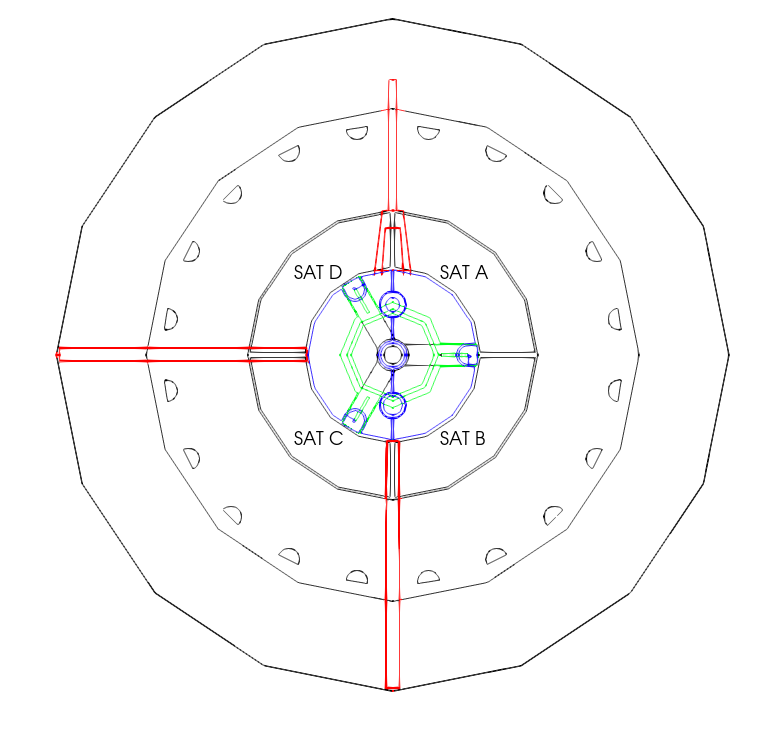
\includegraphics[width=\textwidth]{Figures/Geometry/geometry_with_conduits.png}
\centering
\caption{LZ geometry schematic. The OD geometry excluding the BATs and TATs is shown in black. The BATs and bottom on OCV are shown in green. The TATs, CSD ports and PMT conduits in blue. The DD calibration conduits and the High-Voltage feed through for the TPC are shown in red.}
\label{fig:OD_conduit_geometry}
\end{figure}


\par
As a way of suppressing cavern-$\gamma$'s is to take a slice in $z$, taking events reconstructed to be in the middle of the side tanks.
The resultant pulse area spectrum is shown in \autoref{fig:od_data_pulsearea_middle_tank}.
When compared to \autoref{fig:od_backgrounds_position_reconstruction} additional features appear around 300 phd.
These are consistent with ${}^{60}Co$ which is present in the OCV.
In future it may be possible to accurately measure the rate of this using this volume cut, but that will require a more dedicated calibration campaign, as the true quantity of the SAT selected is not clear.

\begin{figure}[!htbp]
    \centering
    \begin{tikzpicture}
    
    \begin{axis}[
        xlabel=Pulse Area,
        ylabel=Rate (Hz/5phe),
        width=15cm, height=10cm,
        xmin=0, xmax=800,
        ymin=1e-4, ymode=log,
        legend pos=north east,
        grid=major]
            
        \addplot[only marks, mark size=0.5pt] 
            plot[error bars/.cd, x dir=both, x explicit]
            table[x=pulsearea,y=rate,x error=x_error, y error=y_error]
            {Data/OD_Backgrounds/background_constraints/od_data_pulsearea_middle_tank_binwidth_5.dat};
            
        \end{axis}
    \end{tikzpicture}
    \caption{OD pulse area spectrum from pulses reconstructed to the middle of the OD side tanks, suppressing the rate from Cavern-$\gamma$'s.}
    \label{fig:od_data_pulsearea_middle_tank}
\end{figure}


\subsection{$\gamma$ constraints}
\par
Another area to look at is high energy $\gamma$'s, from ($\alpha$,$\gamma$) reactions, which were discussed in \autoref{sec:cavern_gamma_generator}.
In \autoref{fig:od_high_energy} a the expected and observed rate per pulse area above 400 phd is shown.
The rate of events expected is significantly greater than that observed.
The findings here support the discussion in \autoref{sec:cavern_gamma_generator}, that the statistical model used does not extend well to ${}^{17}$O.
However, there are still features seen in data between 1000 and 1800 phd that are not accounted for in simulations.
These features have attributed to neutron captures on the Fe of the water tank (which is made of steel) producing high energy $\gamma$'s \autoref{iron_neutrons_ref}.
These neutrons originate primarily from the ${}^{252}$Cf calibration source, which was stored in a movable safe underground during SR1.
It was moved location within the cavern during SR1 which matches with a change in the reconstructed position of these events.
Backgrounds of this type were not previously considered within LZ, though are of great importance in fusion experiments \cite{iter_neutrons_ref}.
Primarily due to the source safe placement during SR1, it was not possible to determine if there was any fluctuation in the high-energy $\gamma$-rate during SR1.

\begin{figure}[]
    \centering
    \begin{tikzpicture}
    
    \begin{axis}[
        xlabel=Pulse Area (phd),
        ylabel=Rate (Hz),
        width=15cm, height=10cm,
        xmin=400, xmax=3000,
        %ymax=1e-7, 
        ymode=log,
        legend pos=north east,
        grid=major]
            
        \addplot[only marks, mark size=0.5pt,
                 error bar legend,] 
            plot[error bars/.cd, x dir=both, x explicit]
            table[x=pulsearea,y=weight,x error=xerror, y error=yerror]
            {Data/OD_Backgrounds/background_constraints/od_data.dat};
            
        \addplot[red, const plot]
            table [x=pulsearea,y=weight]
            {Data/OD_Backgrounds/background_fit/starting_point/backgrounds_original_purification.dat};
            
        \legend{Data, Expectation};
        \end{axis}
    \end{tikzpicture}
    \caption{OD pulse area spectrum for high energy $\gamma$ events compared to the expected rate.
             The events observed in data between 1000 and 1800 phd are high energy $\gamma$-rays from neutron capture the iron.}
    \label{fig:od_high_energy}
\end{figure}


%%%%%%%%%%%%
\subsection{$\alpha$ constraints}
\par
As was discussed in \autoref{sec:simulated_od_backgrounds} the exact rate of backgrounds from GdLS internals components is not known.
Fortunately we are able to constrain the some of the components. 
The decays within the U and Th decay chains all have an isotope in them with a half-life shorter than the LZ event window, of 4.5 ms.
It will therefore be possible to observe two decays from the same decay chain, which will appear as a pulse-pair (a pulse from each decay).
There are 3 possible decays, one from decay chain ${}^{238}$U, ${}^{235}$U and ${}^{232}$Th.
These are summarised in \autoref{tab:od_constrainable_decays_in_data}.
In reality though, only ${}^{214}$Bi$ \to {}^{214}$Po and ${}^{219}$Rn $\to {}^{215}$Po can be searched for as the interactions from ${}^{212}$Bi $\to {}^{212}$Po are close enough together that they will be merged into one pulse.

\begin{table}[!htbp]
    \centering
    \begin{tabular}{c|c|c|c|c|c}
        \multirow{2}{*}{Decay Pair (chain)}                    & \multicolumn{2}{c|}{First Decay}   & \multicolumn{3}{c}{Second Decay}    \\ 
                                                               & Decay    & Energy (MeV) & Decay    & Energy (MeV) & half-life ($\mu$s) \\ \hline
        ${}^{214}$Bi $\to {}^{214}$Po (${}^{238}$U$_{m}$)          & $\beta$  & 3.27         & $\alpha$ & 7.83         & 160   \\ 
        ${}^{219}$Rn $\to {}^{215}$Po (${}^{235}$U$_{l}$)          & $\alpha$ & 6.95         & $\alpha$ & 7.53         & 1800  \\ 
        ${}^{212}$Bi $\to {}^{212}$Po (${}^{232}$Th$_{l}$)         & $\beta$  & 2.25         & $\alpha$ & 8.95         & 0.3
    \end{tabular}
    \caption{Th and U decay chain pairs with half-lives within the LZ event window of 4.5 ms. 
             Decay information from \cite{radon_chains_ref}.
             See \autoref{fig:decay_chains} for the complete Decay Chains.}
    \label{tab:od_constrainable_decays_in_data}
\end{table}

\par
The decay pairs were searched for by looking for pulses which were reconstructed in be in close proximity to each other.
As the GdLS is not circulated and the decays particles ($\beta$ and $\alpha$) have do not have a significant penetrating power, the site of the two interactions with be very close to each other.
This position requirement acts to reduce the impact of coincident signals in other areas of the OD being mistakenly identified as part of the pulse pair.
The data selection criteria used was simply requiring that the reconstructed $z$ and $\theta$ be within some range of each other: $z_{\text{diff}} < 100$ and $\theta_{\text{diff}} < 1.0$, where diff refers to the difference between pulses.
It was also limited to pulses passing the noise-cut, primarily the PMT multiplicity (coincidence) requirements so that enough PMTs saw light to make the reconstruction meaningful.
This cut is fairly loose to account for potential variable inefficiencies in the position reconstruction with $z$ and $\theta$ based on pulse size.
The resultant pulse-pairs are shown in \autoref{fig:od_all_pulse_pairs_2d}.
Only pulses above 200keV in visible energy are included in the 2D histograms as the features are easier to see.

\begin{figure}[!htbp]%
\centering
\begin{tikzpicture}
\centering
  \begin{axis}[
    height=10cm, width=10cm,
    view={0}{90},
    ylabel={Second Pulse (phd)},
    xlabel={First Pulse (phd)},
    colorbar,
    colorbar style={ylabel={Rate (Hz)},ymode=log,},
    ]
    \addplot3[
      surf,
      shader=flat corner,
	  mesh/cols=40,
	  mesh/ordering=rowwise,
	  point meta = {z<0.0000001 ? nan : z}
    ] file {Data/OD_Backgrounds/background_constraints/rnpo_rate_2d.dat};

  \end{axis}
\end{tikzpicture}
\caption{Relationship of pulses reconstructed in close proximity to each other. Only pulses above 200 keV have been included.}
\label{fig:od_all_pulse_pairs_2d}
\end{figure}

\begin{figure}[!htbp]%
\centering
\begin{tikzpicture}
\centering
  \begin{groupplot}[%view={0}{90},
    group style = {group size = 1 by 2,vertical sep=1.5cm,
                   horizontal sep=1.5cm},
                   height=6cm, width=0.5\textwidth]

	\nextgroupplot[height=10cm, width=10cm,
    view={0}{90},
    ylabel={Second Pulse (phd)},
    xlabel={First Pulse (phd)},
    colorbar,
    colorbar style={ylabel={Rate (Hz)},ymode=log,},
    ]
    \addplot3[
      surf,
      shader=flat corner,
	  mesh/cols=40,
	  mesh/ordering=rowwise,
	  point meta = {z<0.0000001 ? nan : z}
    ] file {Data/OD_Backgrounds/background_constraints/rnpo_rate_2d.dat};
    
    
    \nextgroupplot[height=10cm, width=10cm,
    view={0}{90},
    ylabel={Second Pulse (phd)},
    xlabel={First Pulse (phd)},
    colorbar,
    colorbar style={ylabel={Rate (Hz)},ymode=log,},
    ]
    \addplot3[
      surf,
      shader=flat corner,
	  mesh/cols=40,
	  mesh/ordering=rowwise,
	  point meta = {z<0.0000001 ? nan : z}
    ] file {Data/OD_Backgrounds/background_constraints/bipo_rate_2d.dat};
   
  \end{groupplot}
\end{tikzpicture}
\caption{Relationship of pulses reconstructed in close proximity to each other. Only pulses above 200 keV have been included.
         \textbf{Top:} All pulses-pairs within 800 $\mu$s of each other. The distribution is from ${}^{214}$Bi $\to {}^{214}$Po.
         \textbf{Bottom:} All pulse-pairs with more than 800 $\mu$s time separation between them. The distribution left is from ${}^{219}$Rn $\to {}^{215}$Po.
         }
\label{fig:od_time_dependent_pulses_2d}
\end{figure}



\par
In \autoref{fig:od_bipo_pulses_2d} there is a distribution where both the first and second pulse have a signal size around 170 phd.
These correspond to the double $\alpha$-decay in the ${}^{235}U_{l}$ chain.
The first pulse is slightly smaller than the second, which follows the pattern expected given the $\alpha$ energies shown in \autoref{tab:od_constrainable_decays_in_data}.
The second pulse-pair (from ${}^{238}U_{m}$) has a $\alpha$-decay in the same energy region, $\backsim$170 phd.
The first decay is a $\beta$-decay with the resultant electron have a spectrum of energies up the the end point of 3.27 MeV ($\backsim$ 400 phd).
As such even though the second pulse will be within a small range, there is no clear feature in \autoref{fig:od_bipo_pulses_2d} as the first pulse will be a wide range of values.

\par
It is still possible to isolate ${}^{214}$Bi $\to {}^{214}$Po but taking advantage of the much shorter decay half-life of ${}^{214}$Po vs ${}^{215}$Po.
This was done on the same same data as before with using the same position requirement, except now the time difference between the two pulses is considered.
The of time separation of the pulses has to be less than 800 $\mu$s.
This was selected as it is 5 full half-lives, in which 97\% of all ${}^{214}$Po will have decayed, and is less than half the half-life of ${}^{215}$Po.
The result of this is shown in \autoref{fig:od_time_dependent_pulses_2d}.
Included for completeness as well in \autoref{fig:od_time_dependent_pulses_2d} is the opposite case.
A new distribution has appeared is a second pulse size means of 240 phd, corresponding to the $\alpha$-decay of ${}^{214}$Po.

\par
The distributions in \autoref{fig:od_time_dependent_pulses_2d} allow for the rates of both ${}^{214}$Bi $\to {}^{214}$Po and ${}^{219}$Rn $\to {}^{215}$Po to be constrained.
This gives a rate of 98$\pm$2.5 mHz for ${}^{214}Bi \to {}^{214}Po$ and 7.7$\pm$1.2 mHz for ${}^{219}Rn \to {}^{215}Po$.
Both are rates are lower than those from expected from even the `improved purification' case (discussed in \autoref{sec:simulated_od_requirements}).


\par
Importantly, these constraints indicate that the $\alpha$-peak seen in \autoref{fig:od_random_trigger} is not from those subchains, as the rate would be too low.
This opens up the possibility that it is from ${}^{210}$Po from the late chain of ${}^{238}$U. 
This claim appears at odds with the relatively low internal rate of ${}^{238}$U.
However, it is known and measured that there is significant Rn in the cavern air, and as previously discussed (\autoref{sec:od_construction_sec}) the acrylic tanks were open to the air for long periods prior to installation.
There was opportunity for decay daughters to plate-out on the inside of the acrylic tanks, a feature that is of great concern within the TPC \cite{radon_plateout_ref}.
${}^{210}$Pb is the only long-lived particle in the Radon chain, with a half-life in excess of 22-years. 
The remainder of the isotopes would drastically reduce in abundance after a few weeks, leaving only ${}^{210}$Pb daughters visible, at a sustained rate.
This allows the acrylic holding the scintillator to act as a reservoir, providing a constant supply of $\alpha$ decays from ${}^{210}$Po.
LZ is not alone in having experienced this, with KamLAND measuring a higher than expected rate of ${}^{238}$U$_l$ decays \cite{KamLAND_LS_contaminants_ref}.

\par
The spectra for each of the three visible $\alpha$s are shown in \autoref{fig:od_extracted_alphas}.
The signal size has been converted into visible energy according by the energy scale previously discussed (\autoref{sec:od_energy_scale}).
Although it is unexpected to see a four $\alpha$'s, it becomes possible to perform an $\alpha$ energy calibration, and will be continuously measurable during all Science runs, without the need for Science data taking to be stopped.
An additional advantage is that PMT gain-drift will be more easily detectable.
The observed energy of each of the $\alpha$'s verse the observed energy are shown in \autoref{fig:od_alpha_quenching}, the Birk's law fit is also provided using the parameters in \autoref{tab:Birks_law_parameters}.
It can be seen that the parameters taken from pure LAB remain in good agreement with Gd-doped LAB used here.
This also isolates the difference between observed data and simulations to light propagation.

\begin{figure}[!htbp]%
\centering
\begin{tikzpicture}
\centering
    \begin{axis}[
            ylabel=Rate (Hz/2keV),
            xlabel=Energy (MeV),
            width=15cm,
            height=8cm,
            grid=major,
            xmin=0, xmax=3,
            ymin=1e-4, ymode=log,]
            
        \addplot[red, only marks, mark size=1, 
                 error bars/.cd,
                 y dir=both, y explicit, error bar style={color=black}]
            table [x=energy,y=rate,y error plus index=2, y error minus index=3]
            {Data/OD_Backgrounds/background_constraints/od_bipo_first_alpha.dat};
            
        \addplot[blue, only marks, mark size=1, 
                 error bars/.cd,
                 y dir=both, y explicit, error bar style={color=black}]
            table [x=energy,y=rate,y error plus index=2, y error minus index=3]
            {Data/OD_Backgrounds/background_constraints/od_bipo_second_alpha.dat};
                
    \end{axis}
            
\end{tikzpicture}
    \caption{$\alpha$ energies in from BiPo and RnPo.}
    \label{fig:od_bipo_alphas}
\end{figure}

\begin{figure}[!htbp]%
\centering
\begin{tikzpicture}
\centering
    \begin{axis}[
            ylabel=Visible Energy (MeV),
            xlabel=Particle Energy (MeV),
            width=15cm,
            height=8cm,
            grid=major,
            xmin=0, xmax=10,
            ymin=0,
            legend pos=north west,
            ]
            
        % Birks Fit
        \addplot[red]
            table [x=Energy,y=Quenched]
            {Data/GdLS_Physics/Quenching/alpha.dat};
        \addplot[black, only marks, mark size=1, 
                 error bars/.cd, error bar style={color=black},
                 y dir=both, y explicit,]
            table [x=energy,y=observed,y error plus index=2, y error minus index=3]
            {Data/OD_Backgrounds/background_constraints/od_alpha_energies.dat};
        \legend{Birk's, Measured};
    \end{axis}
            
\end{tikzpicture}
    \caption{Observed energy vs particle energy from $\alpha$ particles.
             The expected quenching from Birk's Law using the parameters in \autoref{tab:Birks_law_parameters} is shown to be in good agreement with what is observed.}
    \label{fig:od_alpha_quenching}
\end{figure}


\subsection{${}^{152}$Gd}
\par
The final background that can be constrained is ${}^{152}$Gd, which produces a 2.2 MeV $\alpha$ decay ($\approx$ 120 keV visible energy).
The GdLS is loaded with 0.1\% (by mass) of natural Gadolinium.
With a total mass of GdLS used in the detector this corresponds to 16000kg, and ${}^{152}Gd$ has a natural abundance of 0.2\%, this gives a maximum possible rate of 27Hz, where there is a 5\% uncertainty on the doping by mass.
\par
Unfortunately this does not constrain does this region entirely.
Of particular note are ${}^{14}$C, a $\beta$ decay with an end-point of 156 keV, and ${}^{147}$Sm which decays via the emission of a 2.3 MeV $\alpha$.
All three were previously measured in the LS screener campaign, with ${}^{14}$C being the dominant contributor (>100 Hz) \cite{scotthaselschwardt_thesis_ref}.


\subsection{Background Fitting}
\par
Using all of the information of the OD backgrounds above, we finish this section is a fit of the expected background to the observed.
Simulations of all of the backgrounds identified in \autoref{sec:simulated_od_backgrounds}, but full light propagation and processed through the same analysis software suite as the observed data.
During this process the simulation signal sizes were scaled by 4.77.
Rather than fitting to the full observable space, a sub range was defined between 20 phd and 600 phd.
The lower limit was set so as to be far enough away from the noise-cut that any uncertainty in scaling factor would not remove these events.
The upper limit was set predominately by the rate of cavern-$\gamma$s.
In this region the expected background rate is 78.43$\pm$2.51 Hz.
This is slightly below the observed rate of 85.26$\pm$0.22 Hz.
\par
In order to keep the number of fit parameters down a number of steps were taken.
Firstly, all detector components were in combined. 
Secondly, contributions from ${}^{152}$Gd and ${}^{147}$Sm were combined together as the energy resolution is not sufficient to separate them.
The cavern-$\gamma$'s were allowed to float within the uncertainties they were measured in \cite{LZ_Gamma_Ray_Background_ref}.
${}^{238}$U$_l$ was allowed to fit between a range of [0, 15] Hz, where 15 is roughly double the size of the integrated rate of the peak at 100 phd above the background rest of the spectra.
${}^{238}$U$_{m}$ and ${}^{235}$U$_{l}$ were constrained by the rates previously reported.
All other backgrounds were left to allowed to float up to the maximum value measured in the LS screener campaign \cite{scotthaselschwardt_thesis_ref}.
\par
The result of the fit is shown in \autoref{fig:od_background_fit_to_data}.
Only components which contributed a more than 0.5 Hz to the OD rate have been included in \autoref{fig:od_background_fit_to_data}, but the fitted line should is from the all contributions.
The individual contributions of each component is shown in \autoref{tab:od_constrainable_decays_in_data}.

\par
${}^{238}$U$_l$ can successfully account for the peak observed at 100 phd, contributing in excess of 8 Hz to the OD rate.
The rate of cavern-$\gamma$s remain the background with the largest uncertainty for the backgrounds in the OD.
There remain some differences between the observed and fitted result, most notably at 50 phd where is a noticeable gap in a background that can fill in this region.
This can be incorporated as an uncertainty in the scaling factor.
The flat scaling of 4.77 did not take into account any position variation, and given that the light collection efficiency observed is significant greater than simulated, it is logical to suggest that the distribution in the LCE map (shown in \autoref{fig:od_lce}) is different as well.
This would effectively make contributions in lower light collection regions appear smaller than they are observed to be, which may go so way to explain what is seen.


\begin{figure}[!htbp]%
\centering
\begin{tikzpicture}
\centering
    \begin{groupplot}[
    group style = {group size = 1 by 2,vertical sep=1.0cm}
    ]
    \nextgroupplot[
            ylabel=Rate (Hz/5phd),
            xlabel=,
            xmajorticks=false,
            width=15cm,
            height=10cm,
            grid=major,
            xmin=0, xmax=700,
            ymin=1e-2, ymax=100,
            ymode=log,
            legend style = { column sep = 10pt, legend columns = 3, cells={line width=1.5pt}}
            ]
        \addplot[only marks, mark size=1.0pt, black, error bar legend] 
            plot[error bars/.cd, x dir=both, x explicit, ]%y dir=both, y explicit, ]
            table[x=pulsearea,y=weight,x error=xerror, y error=yerror]
            {Data/OD_Backgrounds/background_constraints/od_data.dat};
        \addlegendentry{data};
            
        \addplot[const plot, teal]
            table [x=bin_low, y=weight]
            {Data/OD_Backgrounds/background_fit/fit_components/rg_k40.dat};
        \addlegendentry{Cavern ${}^{40}$K};
        \addplot[const plot, cyan]
            table [x=bin_low, y=weight]
            {Data/OD_Backgrounds/background_fit/fit_components/rg_u238.dat};
        \addlegendentry{Cavern ${}^{238}$U};
        \addplot[const plot, green]
            table [x=bin_low, y=weight]
            {Data/OD_Backgrounds/background_fit/fit_components/rg_th232.dat};
        \addlegendentry{Cavern ${}^{232}$Th};
        \addplot[const plot, lime]
            table [x=bin_low, y=weight]
            {Data/OD_Backgrounds/background_fit/fit_components/ocv.dat};
        \addlegendentry{Detector};
        \addplot[const plot, yellow]
            table [x=bin_low, y=weight]
            {Data/OD_Backgrounds/background_fit/fit_components/Internal_improved_u238_early.dat};
        \addlegendentry{${}^{238}$U early};
        \addplot[const plot, pink]
            table [x=bin_low, y=weight]
            {Data/OD_Backgrounds/background_fit/fit_components/Internal_improved_u238_late.dat};
        \addlegendentry{${}^{238}$U late};    
        \addplot[const plot, olive]
            table [x=bin_low, y=weight]
            {Data/OD_Backgrounds/background_fit/fit_components/Internal_improved_th232_early.dat};
        \addlegendentry{${}^{232}$Th early};
        \addplot[const plot, brown]
            table [x=bin_low, y=weight]
            {Data/OD_Backgrounds/background_fit/fit_components/Internal_improved_C14.dat};
        \addlegendentry{${}^{14}$C};
        \addplot[const plot, orange]
            table [x=bin_low, y=weight]
            {Data/OD_Backgrounds/background_fit/fit_components/Internal_improved_Gd152.dat};
        \addlegendentry{${}^{152}$Gd + ${}^{147}$Sm};
        \addplot[const plot, violet]
            table [x=bin_low, y=weight]
            {Data/OD_Backgrounds/background_fit/fit_components/total_fit.dat};
        \addlegendentry{fit};
            
            
    \nextgroupplot[
            ylabel=Ratio (data/fit),
            xlabel=Pulse Area (phd),
            width=15cm,
            height=5cm,
            grid=major,
            xmin=0, xmax=700,
            ymin=0, ymax=2,
            ]
        \addplot[only marks, mark size=1.0pt, black, error bar legend] 
            plot[error bars/.cd, y dir=both, y explicit]
            table[x=bin,y=value, y error=error]
            {Data/OD_Backgrounds/background_fit/fit_components/ratio.dat};
        
        \addplot[black, mark=none, dashed] coordinates {(20,-1) (20,3)};
        \addplot[black, mark=none, dashed] coordinates {(600,-1) (600,3)};
        
    \end{groupplot}
\end{tikzpicture}
    \caption{Result of fit to data.
             \textbf{Top:} Contribution from each source. Only components with a contribution greater than 1 Hz have been included.
             \textbf{Bottom:} Ratio of fit to data. The dashed lines indicate the fit region.
             In generally there is good agreement.}
    \label{fig:od_background_fit_to_data}
\end{figure}


\begin{table}[!htbp]
    \centering
    \begin{tabular}{c|c|c}
        Source               &  Decay Type(s)               & Fitted Rate (Hz) \\ \hline
        \multicolumn{3}{l}{\textbf{Externals}} \\
        Cavern ${}^{238}$U   & $\gamma$                     & 7.65$\pm$1.65                    \\ 
        Cavern ${}^{232}$Th  & $\gamma$                     & 12.94$\pm$3.04                    \\ 
        Cavern ${}^{40}$K    & $\gamma$                     & 12.50$\pm$5.77                    \\ 
        Detector             & $\gamma$,$\beta$             & 3.63$\pm$0.67              \\ \hline
        \multicolumn{3}{l}{\textbf{Internals}} \\
        ${}^{238}$U$_{e}$     & $\gamma$,$\alpha$,$\beta$   & 0.98$\pm$0.21                    \\ 
        ${}^{238}$U$_{m}$     & $\gamma$,$\alpha$,$\beta$   & 0.03$\pm$0.10                   \\
        ${}^{238}$U$_{l}$     & $\gamma$,$\alpha$,$\beta$   & 8.74$\pm$2.34                \\
        ${}^{235}$U$_{e}$     & $\gamma$,$\alpha$,$\beta$   & 0.39$\pm$0.23                    \\
        ${}^{235}$U$_{l}$     & $\gamma$,$\alpha$,$\beta$   & 0.44$\pm$0.12                    \\
        ${}^{232}$Th$_{e}$    & $\gamma$,$\alpha$,$\beta$   & 0.18$\pm$0.04                    \\
        ${}^{232}$Th$_{l}$    & $\gamma$,$\alpha$,$\beta$   & 0.51$\pm$0.08                  \\
        ${}^{40}$K          & $\gamma$,$\beta$              & 0.05$\pm$0.01                 \\
        ${}^{14}$C          & $\beta$                       & 26.97$\pm$7.70           \\
        ${}^{176}$Lu        & $\gamma$,$\beta$              & 0.14$\pm$0.05               \\
        ${}^{147}$Sm and ${}^{152}$Gd    & $\alpha$         & 10.32$\pm$7.24                     
        
    \end{tabular}
    \caption{Fitting contributions of OD backgrounds to the observed data. The reported errors are statistical only.}
    \label{tab:od_constrainable_decays_in_data}
\end{table}

\subsection{Conclusion}
\par
To summarise this section, the OD rate for a number of months.
During this time the OD backgrounds were stable, with the rate above the noise-cut of 276.8 Hz, above 100 keV of 95.8 Hz and above 200 keV as 42.5 Hz.
The rate above 100 keV indicates that a veto time window of 500 $\mu$s is possible.
\par
Several background contributions have been measured in the OD and have been fitted against.
An un-expected contribution from ${}^{238}$U$_{l}$ is present which is believed to be from the radon emanation.
This entered all of the tanks via the frequent opening and closing the valves discussed in \autoref{sec:od_construction_sec}.


%\section{Neutron Efficiency}
\par
For calculating the neutron efficiency during SR1 calibrations, AmLi was used.
As seen in \autoref{sec:sec:od_simulation_efficiency}, the efficiency is no longer expected to meet the requirement of 95\% efficiency.
But, as has been shown in the previous section, the simulation significantly underestimates the light collection efficiency, and so it's possible that the neutron propagation is also not modelled adequately.

\par
Three AmLi sources were used at the same time during this calibration, each placed in a different CSD tube.
This is summarised in \autoref{tab:amli_source_activities}.

\begin{table}[!htbp]
    \centering
    \begin{tabular}{c|c|c}
        CSD & AmLi Source No. & Activity (n/s) \\ \hline
        1   & Source-2        & 13.8           \\
        2   & Source-1        & 9.3            \\ 
        3   & Source-3        & 11.9                
    \end{tabular}
    \caption{AmLi source activities in each CSD}
    \label{tab:amli_source_activities}
\end{table}

\par
For this data, the S2-trigger was used, and the cuts developed for the WIMP search were used to filter out unusable data, to leave a fairly pure dataset of neutron recoils.
These are summarised below, but are detailed in \cite{lz_ws_sr1_ref};

\begin{enumerate}
    \item \textbf{SS}: Single Scatter cut as determined by the interaction finder, shown to be 98.5\% efficient.
    \item \textbf{S2Cuts}: Remove events where the S2 pulse has unusual properties.
    \item \textbf{S1Cuts}: Remove events where the S1 pulse has unusual properties.
    \item \textbf{FID}: Fiducial Volume, to remove wall events and ensure that the neutron penetrated deep enough.
    \item \textbf{NR}: Select events that have nuclear recoiled by selecting events within 1-$\sigma$ of the NR band, which was calibrated using the external DD neutron source.
\end{enumerate}

\par
Three positions in the CSD were used, 0mm, 700mm and 1400mm. 
These definitions are identical to those used in \autoref{sec:od_simulation_efficiency}.
The result of applying the selection cuts to these runs is shown in \autoref{tab:amli_calibration_summary}.

\begin{table}[!htbp]
    \centering
    \begin{tabular}{c|c|c|c|c}
        \multirow{2}{*}{z position (mm)} & \multirow{2}{*}{Run IDs}  & \multicolumn3{c}{Number}  \\ 
                                         &                           & Events    & SS & passing all cuts     \\ \hline
        0                                & 8350-8369                 & 5,504,700 & X  & X               \\
        700                              & 8304-8317                 & 3,688,200 & X  & X               \\ 
        1400                             & 8319-8348                 & 7,041,500 & X  & X                
    \end{tabular}
    \caption{Summary of AmLi source deployment during post SR1 calibrations}
    \label{tab:amli_calibration_summary}
\end{table}

\par
From these events it is then possible to search for events that occur after the S1 in both the Skin and OD.
Those events which pass the TPC cuts are shown in XXX.




\par
Using the maximum veto window for 200keV of 1200$\mu$s, the efficiency as a function of photons detected is shown in \autoref{fig:commissioning_amli_efficiency_per_phd}.
The combined veto efficiency of the Skin and OD are used here due to the limited impact the Skin has on the veto efficiency of neutrons.

\begin{figure}[!htbp]%
\centering
\begin{tikzpicture}
\centering
    \begin{axis}[
            ylabel=Efficiency (\%),
            xlabel=Photons Detected (phd),
            width=15cm,
            height=8cm,
            grid=major,
            xmin=0, xmax=100,
            %ymin=45, ymax=100,
            %minor y tick num=1,
            ]
        \addplot[red,
                 error bars/.cd, error bar style={color=red},
                 y dir=both, y explicit, 
                 x dir=both, x explicit,
                 ]
            table [x=bin,y=value, y error minus index=4, y error plus index=5, x error minus index=2, x error plus index=3,]
            {Data/Neutron_Efficiency/AmLi_Commissioning/pos_0_efficiency_per_phd.dat};    
        \addplot[green, 
                 error bars/.cd, error bar style={color=green},
                 y dir=both, y explicit, 
                 x dir=both, x explicit,
                 ]
            table [x=bin,y=value, y error minus index=4, y error plus index=5, x error minus index=2, x error plus index=3,]
            {Data/Neutron_Efficiency/AmLi_Commissioning/pos_700_efficiency_per_phd.dat};             
        \addplot[blue,
                 error bars/.cd, error bar style={color=blue},
                 y dir=both, y explicit, 
                 x dir=both, x explicit,
                 ]
            table [x=bin,y=value, y error minus index=4, y error plus index=5, x error minus index=2, x error plus index=3,]
            {Data/Neutron_Efficiency/AmLi_Commissioning/pos_1400_efficiency_per_phd.dat};    
        \legend{0mm,700mm,1400mm}  
            
    \end{axis}
            
\end{tikzpicture}
    \caption{Efficiency as a function of pulse area}
    \label{fig:commissioning_amli_efficiency_per_phd}
\end{figure}


\par
Due to the poorer than expected performance of the OD for tagging neutrons, the decision was made to use the longer veto window of 1200$\mu$ combined with a 200keV pulse requirement in the OD or a 100keV requirement in the Skin.
The result of this is summarised in \autoref{fig:commissioning_amli_efficiency_with_bg_rate}.

\begin{figure}[]%
\centering
\begin{tikzpicture}
\centering
    \begin{axis}[
            ylabel=Efficiency (\%),
            xlabel=Time ($\mu$s),
            width=14cm,
            height=8cm,
            grid=major,
            axis y line*=left,
            xmin=0, xmax=1500,
            ymin=45, ymax=100,
            minor y tick num=1,
            legend style = { column sep = 10pt, legend columns = -1,},
            legend pos=north west,
            ]
        \addplot+[red, mark=none, forget plot]
                  table [x=bin,y=value]
                  {Data/Neutron_Efficiency/AmLi_Commissioning/pos_0_od_200kev_efficiency.dat};   
        \addplot[red, only marks, mark size=1.0pt,
                 error bar legend,
                 error bars/.cd, error bar style={color=black},
                 y dir=both, y explicit, 
                 x dir=both, x explicit,
                 ]
            table [x=bin,y=value, y error minus index=4, y error plus index=5, x error minus index=2, x error plus index=3,]
            {Data/Neutron_Efficiency/AmLi_Commissioning/pos_0_od_200kev_efficiency.dat};    
            
        \addplot+[green, mark=none, forget plot]
          table [x=bin,y=value]
          {Data/Neutron_Efficiency/AmLi_Commissioning/pos_700_od_200kev_efficiency.dat};      
        \addplot[green, 
                 only marks, mark size=1.0pt,
                 error bar legend,
                 error bars/.cd, error bar style={color=black},
                 y dir=both, y explicit, 
                 x dir=both, x explicit,
                 ]
            table [x=bin,y=value, y error minus index=4, y error plus index=5, x error minus index=2, x error plus index=3,]
            {Data/Neutron_Efficiency/AmLi_Commissioning/pos_700_od_200kev_efficiency.dat};       
            
        \addplot+[blue, mark=none, forget plot]
          table [x=bin,y=value]
          {Data/Neutron_Efficiency/AmLi_Commissioning/pos_1400_od_200kev_efficiency.dat};         
        \addplot[blue, 
                 only marks, mark size=1.0pt,
                 error bar legend,
                 error bars/.cd, error bar style={color=black},
                 y dir=both, y explicit, 
                 x dir=both, x explicit,
                 ]
            table [x=bin,y=value, y error minus index=4, y error plus index=5, x error minus index=2, x error plus index=3,]
            {Data/Neutron_Efficiency/AmLi_Commissioning/pos_1400_od_200kev_efficiency.dat};    
        \legend{0mm,700mm,1400mm}  
            
    \end{axis}
    \begin{axis}[
            ylabel=False Veto (\%),
            yticklabel pos=right,
            axis y line*=right,
            axis x line=none,
            width=14cm,
            height=8cm,
            %grid=major,
            xmin=0, xmax=1500,
            ymin=0, ymax=50,
            minor y tick num=9,]
        \addplot[domain=0:1500,
            samples=3,
            ]
            {x * 42.5 * 100 / 1000000};
        \iffalse
        \addplot[domain=0:1500,
            samples=3,
            ]
            {x * 95.8 * 100 / 1000000};        
        \addplot[domain=0:1500,
            samples=3,
            ]
            {x * 276.8 * 100 / 1000000};  
        \fi
         \addplot[dashed, mark=none, red] coordinates {(0,5) (1500,5)};
         
        % \node[rotate=24] at (axis cs: 1000,26) {276.8Hz};
        % \node[rotate=11] at (axis cs: 1400,15.5) {95.8Hz};
         \node[rotate=5] at (axis cs: 1400,8) {42.5Hz};
    \end{axis}
            
\end{tikzpicture}
    \caption{Neutron tagging efficiency from AmLi at each height for the 200~keV phe threshold.
    The horizontal dashed line is the 5\% impact on live-time requirement.
    The black line is the 200~keV background rate in the OD.}
    \label{fig:commissioning_amli_efficiency_with_bg_rate}
\end{figure}


\par
On SR1 WIMP-search data, this has a total impact of 4.99\% on live-time, and the resultant events which were vetoed are shown in Figure XXX.
No neutrons were vetoed in SR1 which corresponds to no neutrons being expected.
The events which were vetoed were electron recoil events which were coincidence with an OD background.

\begin{figure}[!htbp]
    \centering
    
\includegraphics[width=0.5\textwidth]{Figures/Placeholder.png}
    \caption{Effect on SR1 data before and after the \textbf{Veto} cut.}
    \label{fig:tpc_with_od_veto_in_sr1}
\end{figure}

\par
The AmLi 

\begin{figure}[]%
\centering
\begin{tikzpicture}
\centering
    \begin{axis}[
            ylabel=Log10(S2) (phd),
            xlabel=S1 (phd),
            width=15cm,
            height=8cm,
            xmin=0, xmax=600,
            ymin=3, ymax=5,
            %ymin=45, ymax=100,
            %minor y tick num=1,
            ]
            
        \addplot[black, only marks, mark=+]
            table []
            {Data/Neutron_Efficiency/AmLi_Commissioning/s1s2_passed_od_veto_in_fid.dat};    
        \addplot[green, only marks, mark=o]
            table []
            {Data/Neutron_Efficiency/AmLi_Commissioning/s1s2_failed_od_veto_in_fid.dat};
        
        \addplot[blue, ]
            table [x=s1c, y=mean]
            {Data/tpc/sr1_er_band.dat};     
        \addplot[blue, dashed]
            table [x=s1c, y=nsig1]
            {Data/tpc/sr1_er_band.dat};     
        \addplot[blue, dashed]
            table [x=s1c, y=psig1]
            {Data/tpc/sr1_er_band.dat};     

        \addplot[red, ]
            table [x=s1c, y=mean]
            {Data/tpc/sr1_nr_band.dat};     
        \addplot[red, dashed]
            table [x=s1c, y=nsig1]
            {Data/tpc/sr1_nr_band.dat};     
        \addplot[red, dashed]
            table [x=s1c, y=psig1]
            {Data/tpc/sr1_nr_band.dat};     
            
    \end{axis}
            
\end{tikzpicture}
    \caption{TPC events vetoed by the OD. In Red are events which passed all cuts including the OD veto. In Blue are events which passed all cuts except the OD veto.}
    \label{fig:sr1_vetoed_events}
\end{figure}


\subsection{Neutron Captures}
\par
Although AmLi 
Another source that can be used to study the neutron capture time is the ${}^{252}{Cf}$ calibration source.
Spontaneous fission of ${}^{252}{Cf}$ typically results in a number of $\gamma$'s with a combined energy of up to 10MeV which are accompanied by a number of neutrons.
An example event from the LZ calibration run pre-SR1 is shown in \autoref{fig:cf252_event_viewer}.
This allows for neutrons to be tagged by tagging the fission by coincident $\gamma$'s in a each detector, and assuming later pulses are dominated by neutrons.

\begin{figure}[!htbp]
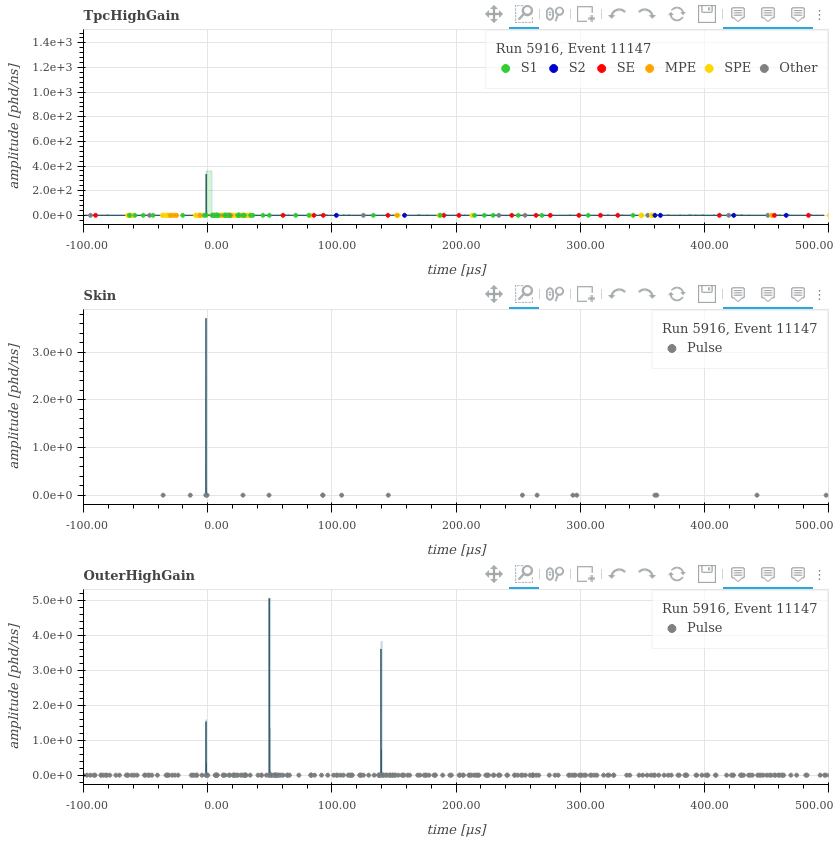
\includegraphics[width=\textwidth]{Figures/NeutronCaptureTime/cf252_eventviewer_5916.png}
\centering
\caption{Example event from ${}^{252}{Cf}$ calibration run showing the $\gamma$'s causing coincident pulses in each detector followed by two neutrons being captured in the Outer Detector}
\label{fig:cf252_event_viewer}
\end{figure}

\par
Although \autoref{fig:cf252_event_viewer} indicates that prompt $\gamma$'s can be used for tagging it does come with a significant caveat; namely that expressed in \autoref{fig:fission_fragments_time}.
There is a non-insignificant probability that $\gamma$'s will be emitted at the same time as a $\gamma$ from a neutron capture is released.
Additionally the majority of study into prompt $\gamma$'s from fission focus on the first 100ns post-fission and the energy and multiplicity beyond that time is not well theorised. 
However, by selecting events which only have a double or triple detector coincidence this can be mitigated.


\begin{figure}[!htbp]
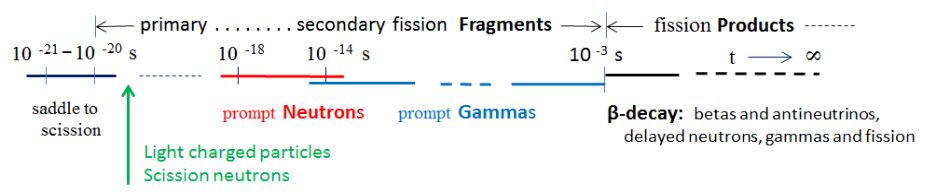
\includegraphics[width=13cm]{Figures/NeutronCaptureTime/fission_fragment_times.png}
\centering
\caption{Emission time-frame of fission components. Adapted from \cite{cf252_fission_ref}}
\label{fig:fission_fragments_time}
\end{figure}

\begin{figure}[]%
\centering
\begin{tikzpicture}
\centering
    \begin{axis}[
            ylabel=Count,
            xlabel=Pulse Area (phd),
            width=15cm,
            height=8cm,
            grid=major,
            xmin=0, xmax=2500,
            ymode=log,
            %ymin=45, ymax=100,
            %minor y tick num=1,
            ]
        \addplot[red, only marks, mark size=1.0,
                 error bar legend,
                 error bars/.cd, error bar style={color=black},
                 y dir=both, y explicit, 
                 x dir=both, x explicit,
                 ]
            table [x=pulsearea,y=weight, x error=xerror, y error=yerror]
            {Data/cf252/cf252_od_pulses_before400ns.dat};    
        \addplot[green, only marks, mark size=1.0,
                 error bar legend,
                 error bars/.cd, error bar style={color=black},
                 y dir=both, y explicit, 
                 x dir=both, x explicit,
                 ]
            table [x=pulsearea,y=weight, x error=xerror, y error=yerror]
            {Data/cf252/cf252_od_pulses_within400ns.dat};           
        \addplot[blue, only marks, mark size=1.0,
                 error bar legend,
                 error bars/.cd, error bar style={color=black},
                 y dir=both, y explicit, 
                 x dir=both, x explicit,
                 ]
            table [x=pulsearea,y=weight, x error=xerror, y error=yerror]
            {Data/cf252/cf252_od_pulses_after400ns.dat};
        \legend{Before 400ns,Within 400ns,After 400ns}  
            
    \end{axis}
            
\end{tikzpicture}
    \caption{Pulse Distribution depending upon when the tagging pulse was.}
    \label{fig:cf252_pulse_selection}
\end{figure}

\begin{figure}[!htbp]%
\centering
\begin{tikzpicture}
\centering
    \begin{axis}[
            ylabel=Count,
            xlabel=Photons Detected (phd),
            width=15cm,
            height=8cm,
            grid=major,
            xmin=0, xmax=2500,
            %ymin=45, ymax=100,
            %minor y tick num=1,
            ]
        \addplot[black, only marks, mark size=1.0,
                 error bars/.cd, error bar style={color=black},
                 y dir=both, y explicit, 
                 x dir=both, x explicit,
                 ]
            table [x=pulsearea,y=weight, x error=xerror, y error=yerror]
            {Data/cf252/cf252_od_largest_after400ns.dat}; 
            
    \end{axis}
            
\end{tikzpicture}
    \caption{Largest OD pulse in an event window 400ns after the first coincidence pulse.}
    \label{fig:cf252_gd152_captures}
\end{figure}

\begin{figure}[]%
\centering
\begin{tikzpicture}
\centering
    \begin{axis}[
            ylabel=Count,
            xlabel=Capture Time ($\mu$s),
            width=15cm,
            height=8cm,
            grid=major,
            ymode=log,
            xmin=-10,xmax=1000,
            ymin=1,
            %minor y tick num=1,
            ]
        \addplot[black, only marks, mark size=0.5,
                 error bars/.cd, error bar style={color=black},
                 y dir=both, y explicit, 
                 x dir=both, x explicit,
                 ]
            table [x=time,y=weight, x error=xerror, y error=yerror]
            {Data/cf252/cf252_gd_capture_time.dat}; 
            
        \addplot[red,
                 domain=15:1500,
                 ]
            {2305 * exp(-x/30.5) + 342 * exp(-x/125.2) + 0.9663}; 
            
        \addplot[blue,
                 domain=15:1500,
                 ]
            {2294 * exp(-x/31.2) + 235 * exp(-x/70.1) + 11.94 * exp(-x/176.4)}; 
            
    \end{axis}
            
\end{tikzpicture}
    \caption{Pulse Distribution depending upon when the tagging pulse was.
             In red is the best fit from 2 exponential decays.
             In blue is the expected neutron capture time.}
    \label{fig:cf252_gd_capture_time}
\end{figure}

\par
The best fit was found to be with just two exponents.
With $t_0 = 31.39 \pm 0.4\mu s$ and $t_1 = 124.5 \pm 1.7\mu s$, with a $\chi^2=0.821$.
$t_0$ accounts for neutrons which travel straight through from the source position to the GdLS and are captured on the GdLS.
$t_1$ is more complex as it accounts for neutrons scatter several times in not the GdLS, such as the acrylic of foam regions.
Given each of these have a different affect on this, it is not clear exactly what is causing it.
This is particularly apparent when compared to the expected result from simulations (also included in \autoref{fig:cf252_gd_capture_time}, where we can see that the neutrons are taking longer than expected to be captured in the OD.
This indicates that neutrons are becoming trapped in materials between the calibration tube and the OD.
The possible materials between the CSD and the OD are primarily foam, acrylic and water.
Given that the acrylic thickness was measured during construction, this leaves water as the most likely scenario.

\par
One possible reason for this is the foam surrounding the OCV not stopping all water from coming into that region.
Though when the SATs were installed, there was no discernible gap between the SAT and the Tyvek around the OCV foam.
Though it is possible that a small amount of water would have entered this area over time, but no more than a few mm.

\par
Another possibility is that the foam became at least in part filled with water.
Water ingress in foam has been well studied at least in part, with the industrial measures of water absorption defined as via diffusion and by submersion \cite{foam_with_water_ref}.
The effectiveness of any foam type to keep water out is based on a number of factors including density and most importantly if the structure is closed or open\footnote{in terms of whether the cells which make up the foam structure. Open cell foams are softer and more flexible as each cell is open to the atmosphere. Closed cell foams are firmer with the majority of cells being closed to the atmosphere.}.
The difference in terms of water ingress is shown in \autoref{fig:foam_mri_water_ingress}.


\begin{figure}[!tbhp]
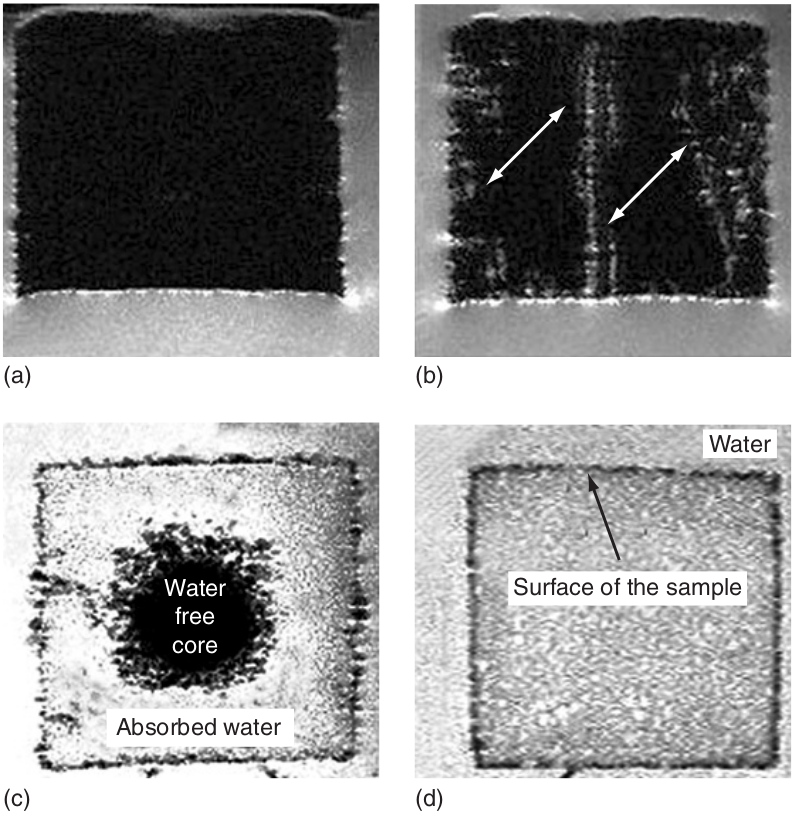
\includegraphics[width=\textwidth]{Figures/NeutronCaptureTime/foam_water_absorption.png}
\centering
\caption{Magnetic resonance images of 30 mm cube samples of polyurethane foam for two types of different foam of the same density, 0.3 g m${}^{-3}$: a closed cell foam (top) and an open cell foam (bottom).
(a) closed cell foam after 8 hours. (b) closed cell foam after 63 hours.
(c) open cell foam after 8 hours. (d) open cell foam after 72 hours.
Images from \cite{foam_mri_data_ref}.
}
\label{fig:foam_mri_water_ingress}
\end{figure}


\par
The foam installed around the OCV (green foam in \autoref{sec:od_construction_sec}) is a closed cell foam expanded using $CO_2$, so each cell is filled with $CO_2$, foam 3000 CS in \cite{styrodur_water_ingress_ref}.
As such the foam is expected to experience a 0.7\% volume ingress of water due to long term submersion and 5\% volume ingress of water from diffusion\footnote{long-term in this case refers to a 28-day test as is the industry standard, see BS EN ISO 16535 (previously BS EN 12087) and BS EN ISO 16536 (previously BS EN 12088).}.
These values, being based off of tests designed of industry do not necessarily map obviously onto how it was used in this application, particularly given that water pressure is not considered in the industrial tests and the long-term are orders of magnitude less than the exposure the LZ foam has had already.
\par
In order to begin probing this, a test was conducted to observe what happens to this foam (and what happens to the water).
An example of each piece of foam used, was placed in de-ionised water and placed under a $N_2$ purge. 
The water resistivity was measured every few hours as a monitor of the water's purity.
The result over the first week of running is shown in \autoref{fig:od_foam_degredation}.
What is observed during this period is the water becoming contaminated with ions from the foam from out gassing.
Over a longer period of study it may show that the foam becomes saturated with water, particularly with a test using a piece of foam shaped to the same dimensions as those used in the installation.
\par
The foam installed between the TATs and OCV are held together with HandiFoam\textsuperscript{\textregistered}, which also forms a closed cell structure: not only does the outer layer is enclosed everything, but the inner structure is 95\% closed cell.
However, due to it's low-pressure it is classified as "vapour retardant", and prolonged exposure to water will rapidly saturate the foam \cite{handifoam_water_ingress_ref}.
The speed at which this occurred was likely accelerated by the cutting into the outer layer, done to shape the foam to size.
\par
The other foam of concern is the polyethylene foam \cite{white_foam_ref}, which is also a closed-cell structure, though with a much finer cell structure.
Though as it's purpose was primarily padding, and the quantity installed is low, water displacement is of less concern.
Only around the BATs is a neutron able to reach the foam before reaching the GdLS.

\par
In relation to LZ, this has two impacts, firstly these ions can circulate throughout the OD water and contribute to the low energy rate.
Secondly, this will impact on the time it takes for a neutron to reach the GdLS.
Taking the most extreme case as the foam being completely replaced with water, we can see that the neutron time to reach the GdLS is significantly increased (shown in blue in \autoref{fig:data_vs_sim_gd_capture_time}).
This therefore seems an reasonable explanation for the difference observed, though some tuning is required for a closer match between the simulation and observed.


\begin{figure}[]%
\centering
\begin{tikzpicture}
\centering
    \begin{axis}[
            xlabel=Time (hours),
            ylabel=Resistivity (mS/cm),
            width=15cm,
            height=8cm,
            grid=major,
            xmin=-1, xmax=250,
            legend style={at={(0.95,0.5)},anchor=east},
            %ymin=45, ymax=100,
            %minor y tick num=1,
            ]
        \addplot[green, only marks,
                 error bars/.cd, error bar style={color=black},
                 y dir=both, y explicit, 
                 ]
            table [x=time,y=di,y error=error]
            {Data/cf252/foam_in_di_water.dat}; 
        \addplot[blue, only marks,
                 error bars/.cd, error bar style={color=black},
                 y dir=both, y explicit, 
                 ]
            table [x=time,y=foam,y error=error]
            {Data/cf252/foam_in_di_water.dat}; 
        \addplot[red, dashed,
                 domain=-10:750,
                 samples=3]
                {1};
            
        \legend{Control, Foam,};
    \end{axis}
            
\end{tikzpicture}
    \caption{Measure of water purity from foam used in the OCV.
             Both the Control (just water) and the Foam (water with foam pieces) were under $N_2$ purge for the duration of the data taking.
             The dashed red line indicated the Type 2 DI water limit.}
    \label{fig:od_foam_degredation}
\end{figure}

\begin{figure}[]%
\centering
\begin{tikzpicture}
\centering
    \begin{axis}[
            ylabel=Count (Arb.),
            xlabel=Capture Time ($\mu$s),
            width=15cm,
            height=8cm,
            grid=major,
            ymode=log,
            xmin=-10,xmax=800,
            ymin=1e-3, ymax=5,
            %minor y tick num=1,
            ]
        \addplot[black, only marks, mark size=0.5,
                 error bars/.cd, error bar style={color=black},
                 y dir=both, y explicit, 
                 ]
            table [x=time,y=weight, y error=yerror]
            {Data/cf252/cf252_gd_capture_time_normed.dat}; 
            
        \addplot[red, const plot]
            table [x=time,y=weight]
            {Data/cf252/amli_0mm_default.dat}; 
            
        \addplot[green, const plot]
            table [x=time,y=weight]
            {Data/cf252/amli_0mm_water_saturated.dat}; 

        \addplot[blue, const plot]
            table [x=time,y=weight]
            {Data/cf252/amli_0mm_water.dat}; 
            
    \end{axis}
            
\end{tikzpicture}
    \caption{Neutron capture time on Gadolinium in the OD. The observed capture time from ${}^{252}$Cf is shown in black. In red is the expected capture time from simulation. In green is the capture time if the foam has been saturated with water up to 5\% of its volume. In blue is the capture time if all foam around the OCV has been replaced with water. Each distribution has been normalised the maximum value.}
    \label{fig:data_vs_sim_gd_capture_time}
\end{figure}


\section{Particle Discrimination}
\par
As previously mentioned, the OD has been designed to act as an "active but dumb" veto.
It could be improved by including some form of interaction identification in the OD.
For example, the Bi-Po interactions in Section XXX can be identified from two interactions in close proximity to each other with relative ease.
These events could then be un-vetoed; increasing the number of candidate events as well as the live-time.

\par
There is also the possibility of discriminating between high energy backgrounds such as neutron captures and cavern-$\gamma$'s.
This would actually be a discrimination between 1-$\gamma$ vs multiple $\gamma$'s.
The viability of this discrimination in simulated datasets is explored in this section.


\subsection{Maximum Likelihood Method}
\par
\par
An important point to note is that the ability of any method to discriminate different event types is how the input variables are selected.
Ideally, each of the input variables would not be correlated with each other.
This is not the case, particularly as we have limited ourselves to using reduced quantities rather than raw waveforms.
So rather than doing pulse-shape discrimination, we are looking at some pre-extracted quantities of a given pulse.

\par
In shorterned form. 
For a given event, the likelihood for being of signal type is obtained by multiplying the signal probability densities of all input variables which are assumed to be independent and normalising this by the sum of the signal and background likelihoods.
Because correlations among the variables are ignored, this PDE approach is also called "naive Bayes estimator" \cite{TMVA_ref}.

Following the style of \cite{TMVA_ref}, the likelihood ratio $y_{\Lagrangian}$ of any event is defined as;
\begin{equation}
    y_{\Lagrangian} = \frac{\Lagrangian_{S}}{\Lagrangian_{S} + \Lagrangian_{B}}
\end{equation}
where
\begin{equation}
    \Lagrangian_{S,(B)} = \prod_k p_{S,(B),k}(x_k)
\end{equation}
where $p_{S,(B),k}$ is the signal (background) PDF for the $k^{th}$ input variable $x_k$.


\subsection{Variables}
\par
A set of simulations were performed using full-chain propagation; particle propagation and PMT modelling.
The resultant waveforms were passed to the reconstruction package.
From the reconstruction, 3 variables were selected to describe a pulse.
The variables, which are described below, were chosen as they are relatively simple.
Meaning that there has been limited manipulation of the raw event data.
Figure XXX shows the variables against one another for a variety of sources.


\paragraph{coincidence}
Sometimes referred to as pulse multiplicity, the coincidence value of a pulse is the number of PMTs which produced a signal that contributed to the pulse.
As the more photons produced, the more will be detected, and so the more likely is it that any given PMT will see this light.
It is a very robust and simple variable, and therefore ideal to start with.
A neutron capture will likely have a higher coincidence as the multiple $\gamma$'s can scatter in different areas of the OD.


\paragraph{pulse area}
The number of photons detected is directly proportional to the energy of the interaction that occurred.
Combined with the coincidence, it has the potential to isolate unwanted pulses such as those caused by PMT after-pulsing.


\paragraph{$\frac{\text{width}}{\text{pulse area}}$}
This variable is the most complicated of the selection, which gives a pulse-shape.
The width of a pulse is the time.
Due to pulse finding limitations, the full reconstructed pulse width was not used.
Instead, the pulse start time was defined as; the time where 5\% of the pulse integral was reached, and the end time as 75\% of the pulse integral.

However, the quantity can be improved by combining it with a second variable; the pulse area.
This has the advantage of removing the pulse area as an influencing parameter in the value and making the variable more stable.
In the simplest case, the quantity gives is how fast or slow the pulse decreases after the peak.
An example of different interactions with this variable can be found in Figure XXX.

\begin{figure}[!htbp]
    \centering
    
\includegraphics[width=0.5\textwidth]{Figures/Placeholder.png}
    \caption{Variables used for particle discrimination}
    \label{fig:discrimination_variables}
\end{figure}

\begin{figure}[]%
\centering
\begin{tikzpicture}
\centering
    \begin{groupplot}[%view={0}{90},
    group style = {group size = 1 by 3,vertical sep=1.5cm}]
    \nextgroupplot[
            xlabel=Pulse Area,
            ylabel=Proportion,
            width=15cm, height=6cm,
            xmin=0, xmax=1000,
            ymin=0,% ymax=100,
            %minor y tick num=4,
            grid=major,
            legend style = { column sep = 10pt, legend columns = -1, legend to name = Simulated_Likelihood_Variables_CommonLegend,}]
            \addplot[green, mark=none]
                    table [x=Centre,y=Normed]
                    {Data/OD_Likelihood/gd_capture_pulseArea_phd.dat};
            \addplot[blue, mark=none]
                    table [x=Centre,y=Normed]
                    {Data/OD_Likelihood/h_capture_pulseArea_phd.dat};
            \addplot[red, mark=none]
                    table [x=Centre,y=Normed]
                    {Data/OD_Likelihood/rockgamma_pulseArea_phd.dat};
            %\node[] at (axis cs: 800,87) {\large 0 mm};
            \legend{Gd-capture,H-capture,Cavern $\gamma$}
        
        \nextgroupplot[
            xlabel=N. PMTs,
            ylabel=Proportion,
            width=15cm, height=6cm,
            xmin=0, xmax=120,
            ymin=0, %ymax=100,
            %minor y tick num=4,
            grid=major,]
            \addplot[green, mark=none]
                    table [x=Centre,y=Normed]
                    {Data/OD_Likelihood/gd_capture_coincidence.dat};
            \addplot[blue, mark=none]
                    table [x=Centre,y=Normed]
                    {Data/OD_Likelihood/h_capture_coincidence.dat};
            \addplot[red, mark=none]
                    table [x=Centre,y=Normed]
                    {Data/OD_Likelihood/rockgamma_coincidence.dat};
            %\node[] at (axis cs: 800,87) {\large 1400 mm};
        \nextgroupplot[
            xlabel=Pulse Time / pulse Area,
            ylabel=Proportion,
            width=15cm, height=6cm,
            xmin=0, xmax=2,
            ymin=0, %ymax=100,
            %minor y tick num=4,
            grid=major,]
            \addplot[green, mark=none]
                    table [x=Centre,y=Normed]
            {Data/OD_Likelihood/gd_capture_areaFractionTime75_ns_vs_pulseArea_phd.dat};
            \addplot[blue, mark=none]
                   table [x=Centre,y=Normed]
              {Data/OD_Likelihood/h_capture_areaFractionTime75_ns_vs_pulseArea_phd.dat};
            \addplot[red, mark=none]
                    table [x=Centre,y=Normed]
                    {Data/OD_Likelihood/rockgamma_areaFractionTime75_ns_vs_pulseArea_phd.dat};
            %\node[] at (axis cs: 800,87) {\large 1400 mm};
             
    \end{groupplot}
    \node at ($(group c1r1) + (-0.5cm, 3.0cm)$) {\ref{Simulated_Likelihood_Variables_CommonLegend}};
\end{tikzpicture}
    \caption{Parameter-space population for various interactions.}
    \label{fig:simulated_likelihood_variables}
\end{figure}

\subsection{Performance}
\par
For this study, the signal was selected to be neutron captures and the background as cavern-$\gamma$'s
The neutron captures were simulated by starting thermalised neutrons in the GdLS.
This meant that only the energy deposits in the OD as a result post-capture were detectable.
The 
\par
The likelihood was performed against a set of simulations which contained a mixture of both neutron captures and cavern-$\gamma$'s in quantities expected \cite{LZ_assay_ref}.
The neutrons were, as above, thermalised so the only interaction of note are from the result of neutron captures.






\begin{figure}[!htbp]
    \centering
    
\includegraphics[width=0.5\textwidth]{Figures/Placeholder.png}
    \caption{ROC curve of}
    \label{fig:discrimination_performance}
\end{figure}

\par
Although it is possible to use this method with data, it has been impractical given the differences mentioned earlier in this Chapter.
In order to perform this, a data-driven approach is required and simulation corrections implemented.
Both of which have not been performed due to time constraints.





\par
Interaction discrimination based upon a likelihood has the potential to improve the OD effectiveness; reducing the dead-time as as result of false vetoes.
It can also reduce the uncertainties on backgrounds - particularly if combined with detector coincidences on Gd-captures as was done in Section XXX.
There is scope for additional interesting studies such as seasonal modulation in rates of interactions such as ($\alpha$,$\gamma$) \cite{cavern_gammas_in_Soudan_mine_ref}.
All of these together can directly improve the sensitivity of LZ to a potential dark matter detection.

\par
Once data is better understood, it may be possible to implement higher dimensional variables to discriminate interactions.
Though all of these are subject to an eventual match-up in simulation and data.
